\documentclass{standalone}
\usepackage{tikz}
\begin{document}
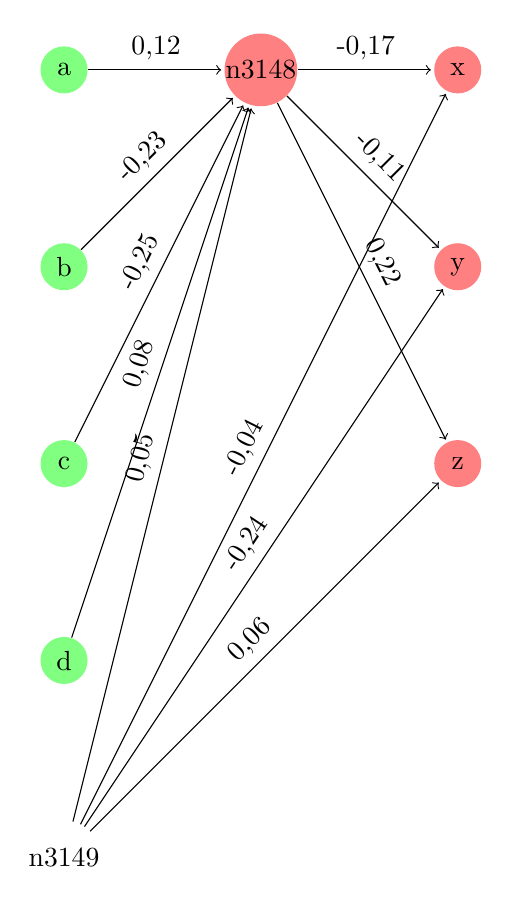
\begin{tikzpicture}[shorten >=1pt,->,draw=black!,node distance=2.5cm]
\tikzstyle{neuron}=[circle,fill=black!25,minimum size=17pt,inner sep=0pt]
\tikzstyle{constant}=[neuron, fill=white!50];
\tikzstyle{identity}=[neuron, fill=green!50];
\tikzstyle{sigmoid}=[neuron, fill=red!50];
\node [identity] (a) {a};
\node [identity,below of=a] (b) {b};
\node [identity,below of=b] (c) {c};
\node [identity,below of=c] (d) {d};
\node [constant,below of=d] (n3149) {n3149};
\node [sigmoid,right of=a] (n3148) {n3148};
\node [sigmoid,right of=n3148] (x) {x};
\node [sigmoid,below of=x] (y) {y};
\node [sigmoid,below of=y] (z) {z};
\path[every node/.style={sloped,anchor=south,auto=false}]
(d) edge node {0,08} (n3148)
(c) edge node {-0,25} (n3148)
(n3148) edge node {-0,17} (x)
(n3148) edge node {0,22} (z)
(n3148) edge node {-0,11} (y)
(n3149) edge node {0,05} (n3148)
(n3149) edge node {-0,04} (x)
(n3149) edge node {-0,24} (y)
(n3149) edge node {0,06} (z)
(b) edge node {-0,23} (n3148)
(a) edge node {0,12} (n3148)
;\end{tikzpicture}
\end{document}